\documentclass{article}

\usepackage[margin=0.5in]{geometry}
\usepackage{multicol}
\usepackage{tikz}
\usepackage{graphicx}

\title{Solid Geometry Set B}
\author{}
\date{}

\begin{document}
\maketitle
\noindent Problems should be solved without calculators unless otherwise specified.
Remember to explain how you solved a problem.
\begin{multicols}{2}
    \begin{enumerate}
        \item What is the total surface area of a right square pyramid with a height of $12$ feet and a base with side length of $10$ feet?
            \vspace{3cm}
        \item This figure shows the net of a three-dimensional shape called a truncated octahedron.
            How many vertices does a truncated octahedron have?
            \begin{center}
                \includegraphics[scale=0.5]{truncated_octahedron.png}
            \end{center}
            \vspace{3cm}
        \item A sphere is inscribed in a cube.
            What is the ratio of the volume of the cube to that of the sphere?
            Express your answer as a common fraction in terms of $\pi$.
            \vspace{3cm}
        \item In the figure shown, a triangular pyramid has been cut off the corner of the cube so that an equilateral triangle face is formed.
            If each corner of the cube is cut off in this manner, what is the maximum sum of the number of faces, edges, and vertices on the new polyhedron?
            \begin{center}
                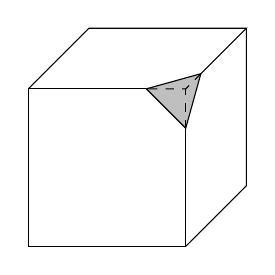
\begin{tikzpicture}[scale=0.5]
                    \draw (3,4,4) -- (0,4,4) -- (0,0,4) -- (4,0,4) -- (4,3,4);
                    \draw (0,4,4) -- (0,4,0) -- (4,4,0) -- (4,4,3);
                    \draw (4,4,0) -- (4,0,0) -- (4,0,4);
                    \draw[fill=lightgray] (4,4,3) -- (3,4,4) -- (4,3,4) -- cycle;
                    \draw[dashed] (4,4,3) -- (4,4,4) -- (3,4,4);
                    \draw[dashed] (4,3,4) -- (4,4,4);
                \end{tikzpicture}
            \end{center}
            \vspace{3cm}
        \item When a cone's height is decreased by a factor of four, to maintain the same volume, the radius must be increased by a factor of two, or $100\%$.
            When the cone's height is decreased by a factor of three, by what percent must the radius be increased to maintain the same volume?
            Express your answer to the nearest whole number.
            \vspace{3cm}
    \end{enumerate}
\end{multicols}
\end{document}
